\documentclass{article}
\usepackage[T1]{fontenc}
\usepackage{lmodern}
\usepackage{graphicx}
\usepackage{amsmath,amssymb}
\usepackage[a4paper,margin=2cm]{geometry}
\usepackage[absolute,overlay]{textpos}
\setlength{\TPHorizModule}{1mm}
\setlength{\TPVertModule}{1mm}
\usepackage[indonesian]{babel}
\usepackage{hyperref}
\setlength{\emergencystretch}{2em}
% unit: Halaman 35

\begin{document}

% === Halaman 35 (llm) ===

\vspace{193.05mm}

\begin{itemize}
    \item Contoh: jika LFSR 4-bit diinisialisasi dengan $U = 1111$
\end{itemize}

\vspace{10mm}

\begin{itemize}
    \item Barisan bit acak: $1\ 1\ 1\ 1\ 0\ 1\ 0\ 1\ 1\ 0\ 0\ 1\ 0\ 0\ 0\ \dots$
    \item Periode LFSR n-bit: $2^n - 1$
\end{itemize}

% deskripsi: Tabel yang menunjukkan proses perubahan isi register dan bit keluaran dari LFSR 4-bit selama 15 siklus (i=0 hingga i=15).
% bbox normalisasi: [0.2200, 0.1300, 0.6400, 0.7800]
\begin{textblock*}{88.20mm}(46.20mm,38.61mm)
\noindent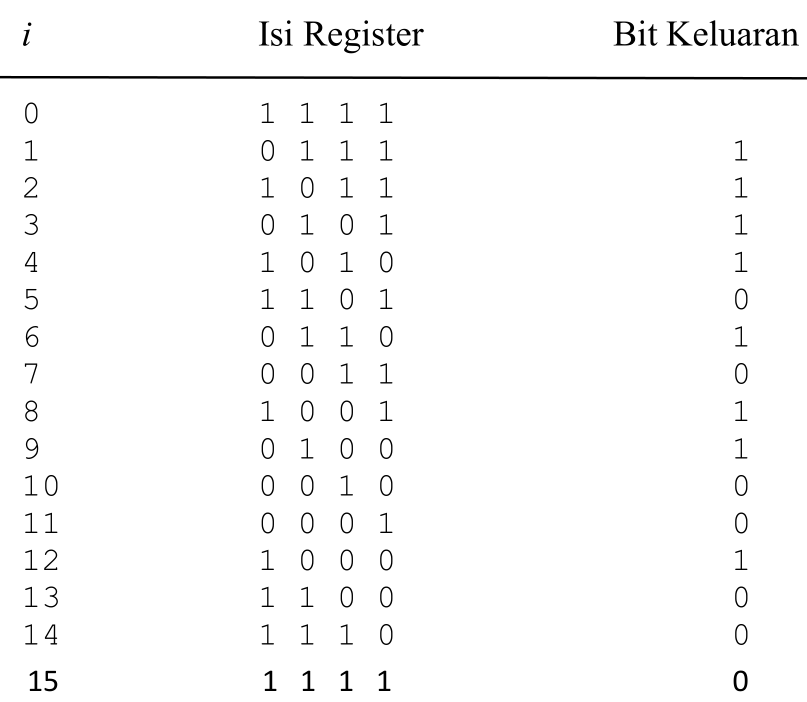
\includegraphics[width=88.20mm,height=193.05mm]{../../images/llm/page_035_img_01.png}%
\end{textblock*}

\end{document}
